
\hfill\break
\justifying
Manteniendo en mente las condiciones del proyecto, se eligió a corde un conjunto de datos para el entrenamiento y prueba de los métodos experimentados. El conjunto de datos elegido \textit{GesturePebble}, se deriva del trabajo \textit{"Gestures Recognition using Symbolic Aggregate Aproximation and Dynamic Time Warping on Motion Data"}[13], el conjunto de datos se encuentra disponible para su uso público en el repositorio de series temporales \textit{UCR Archive}[7].

\hfill\break
\justifying
Incluye instances de series temporales con longitud varible, razón por la que el archivo provisto por UCR, se encuentra acompletado a una longitud de 456 mediciones por patrón con el uso de NaNs en las instancias con menor longitud. Así mismo las etiquetas de clase se colocan como el primer elemento de cada secuencia para un fácil manejo.

\hfill\break
\justifying
Enfocado en el estudio de dispositivos cotidianos como celulares y \textit{wearables} para el reconocimiento de gestos, los datos recolectados son muestreados con las mediciones ofrecidas por el acelerómetro del reloj inteligente Pebble, en los ejes tridimensionales al ser utilizado sobre la muñeca por los sujetos participantes en la generación del conjunto de datos.

\hfill\break
\justifying
El \textit{dataset} involucra a 4 participantes, cada uno instruido para realizar 6 gestos(Figura 1) que repitieron durante un par de sesiones separadas entre días para conseguir un total de 8 grabaciones y completo el \textit{dataset} a un total de 304 gestos. 

\hfill\break
\begin{minipage}{\linewidth}
	\centering
	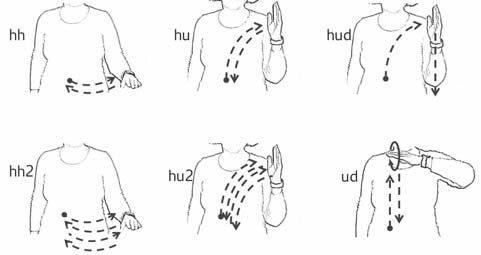
\includegraphics[width=7.5cm]{Imagenes/gestos_motrices.png}
	\label{gestos_motrices}
	\captionof{figure}{Elección de los 6 gestos sencillos etiquetados y realizados por los participantes para la generación de las secuencias temporales disponibles en el \textit{dataset} \textit{GesturePebble}}
\end{minipage}

\hfill\break
\justifying
De las series temporales captadas, se proveén las mediciones del sensor acelerómetro en el eje Z únicamente, facilitando a su vez un par de conjutos de datos con características específicas cada uno: \textit{GesturePebbleZ1} y \textit{GesturePebbleZ2}.

\hfill\break
\justifying
El conjunto de datos \textit{GesturPebbleZ1}, provee un archivo con instancias para el entrenamiento del modelo clasificador, componíendose los patrones desarrollados por los partipantes durante la primer sesión. Mientras que el archivo de prueba, es la colección de los patrones realizados en la segunda sesión.

\hfill\break
\justifying
Para el conjunto \textit{GesturePebbleZ2}, el conjunto de entrenamiento consiste en los datos de un par de sujetos, y el de prueba del par restante. Presumiblemente esta segunda colección está destinado a ser más compleja en dificultad que el primero, impidiendo que el modelo sea entrenado con patrones de los sujetos que más tarde serán evaluados. La dificultad de este \textit{dataset} se argumenta basándose en el hecho de que cada participante posé una postura y mecánica de movimiento distinta a las de los demás.